% !TEX root = saveliev_physics_general_course_1.tex
%!TEX TS-program = pdflatex
%!TEX encoding = UTF-8 Unicode


\chapter{THÔNG TIN CHUNG}\label{chap:10}

\section{Vật lý thống kê và Nhiệt động lực học}\label{sec:10_1}

Vật lý phân tử là một nhánh của Vật lý nghiên cứu cấu trúc và cấu trúc của một chất trên cở sở động học phân tử. Theo các khái niệm này, bất kì vật gì-rắn, lỏng, hoặc khí-bao gồm một số lượng lớn các hạt riêng biệt cực nhỏ-các phân tử. (Các nguyên tử có thể coi là các phân tử đơn nguyên tử ) Các phân tử ở mọi chất đều chuyển động hỗn loạn, mất trật tự và không có hướng chủ đạo. Cường độ chuyển động phụ thuộc vào nhiệt độ của chất.

Một bằng chứng trực tiếp về sự chuyển động hỗn loạn của các phân tử là chuyển động Brown. Hiện tượng này là các hạt rất nhỏ (chỉ nhìn qua kính hiển vi) lơ lửng trong chất lỏng luôn luôn ở trạng thái chuyển động hỗn loạn không ngừng, không phụ thuộc vào các nguyên nhân bên ngoài và là một biểu hiện của chuyển động bên trong vật chất. Chuyển động Brown của các hạt là do sự va chạm hỗn loạn của chúng với các phân tử.

Hướng nghiên cứu của thuyết động học phân tử là giải thích được tính chất của các vật được quan sát trực tiếp được trên thí nghiệm (áp suất, nhiệt độ,v.v...) như là kết quả tác dụng tổng hợp của các phân tử. Đồng thời nó sử dụng phương pháp thống kê, bằng cách không quan tâm đến sự chuyển động của các phân tử riêng biệt mà chỉ quan tâm đến các đại lượng trung bình đặc trưng cho chuyển động của một tổ hợp khổng lồ các hạt. Từ đấy, nó có tên gọi khác là Vật lý thống kê.

Nhiệt động lực học cũng nghiên cứu các tính chất khác nhau của các vật và sự biến đổi trạng thái của các chất. Tuy nhiên, không giống với thuyết động học phân tử, nhiệt động lực học nghiên cứu các đặc tính vĩ mô của các vật thể mà không quan tâm đến bức tranh vi mô của chúng. Nhiệt động lực học cho phép chúng ta đi đến một số lượng đáng kể các kết luận về cách các quá trình diễn ra mà không cần xem xét các phân tử và nguyên tử và không xem xét các quá trình từ quan điểm vi mô.

Nhiệt động lực học được thành lập dựa trên một số định luật cơ bản được thiết lập là kết quả của việc khái quát hóa một lượng lớn các sự kiện thực nghiệm. Do đó, các kết luận của nhiệt động lực học có tính chất rất tổng quát.

Bằng cách xem xét sự thay đổi trạng thái của một chất từ các quan điểm khác nhau, nhiệt động lực học và thuyết động học phân tử sẽ bổ sung lẫn nhau, tạo thành một tổng thể duy nhất về bản chất.

Chuyển sang lịch sử phát triển của các khái niệm động học phân tử, trước hết chúng ta phải chỉ ra rằng những ý tưởng về cấu trúc nguyên tử của một chất đã được người Hy Lạp cổ đại đưa ra. Tuy nhiên, những ý tưởng này không hơn gì một phỏng đoán tuyệt vời. Vào thế kỷ 17, nguyên tử học lại được đặt lên hàng đầu, nhưng với tư cách là một giả thuyết khoa học thay vì phỏng đoán. Giả thuyết này được phát triển đặc biệt lớn trong các công trình của nhà khoa học Nga lỗi lạc Mikhail Lomonosov (1711-1765). Ông đã cố gắng đưa ra một bức tranh duy nhất về tất cả các hiện tượng vật lý và hóa học đã biết vào thời của ông. Ông tiến hành từ khái niệm hạt (theo thuật ngữ hiện đại-phân tử) về cấu trúc của vật chất. Nổi dậy chống lại lý thuyết về sinh nhiệt (một chất lỏng nhiệt giả định có thành phần trong một vật xác định mức độ nóng lên của nó) thịnh hành vào thời của ông, Lomonosov đã nhìn ra "nguyên nhân sinh nhiệt" trong chuyển động quay của các hạt trong vật. Do đó, Lomonosov về bản chất đã hình thành các ý tưởng động học phân tử.

  Vào nửa sau của thế kỷ 19 và đầu thế kỷ 20, nguyên tử học đã trở thành một lý thuyết khoa học nhờ các công trình của một số nhà khoa học.

\section{Khối lượng và kích thước của phân tử}\label{sec:10_2}

Khối lượng của các nguyên tử và phân tử được đặc trưng bằng cách sử dụng các đại lượng được gọi là \textbf{khối lượng nguyên tử tỉ đối của một nguyên tố} (nói gọn là khối lượng nguyên tử) và \textbf{khối lượng phân tử tỉ đối của chất} (nói gọn là khối lượng phân tử). (Những đại lượng này trước đây được gọi là trọng lượng nguyên tử và trọng lượng phân tử)

Khối lượng nguyên tử ($\amr$) của một nguyên tố hóa học là tỷ số khối lượng của một nguyên tử của nguyên tố đó với $1/12$ khối lượng của nguyên tử \ce{C^12} (đồng vị Carbon với số khối lượng \num{12} được ký hiệu như vậy). Khối lượng phân tử ($\mmr$) của một chất là tỷ số khối lượng của một phân tử của chất đó với $1/12$ khối lượng của một nguyên tử \ce{C^12}. Như suy ra từ định nghĩa của chúng, các khối lượng nguyên tử và phân tử là các đại lượng không thứ nguyên.

Đơn vị khối lượng bằng $1/12$ khối lượng của một nguyên tử \ce{C^12} được gọi là \textbf{đơn vị khối lượng nguyên tử} (\textbf{\si{\atomicmassunit}}). Ta ký hiệu đơn vị này được biểu thị bằng Kilogam là $\amu$. Khi đó, khối lượng của một nguyên tử được biểu thị bằng Kilogam sẽ bằng $\amr\amu$, và khối lượng của một phân tử sẽ bằng $\mmr\amu$.

Lượng chất, trong đó có chứa số hạt (các nguyên tử, các phân tử, các ion, các electron và v.v..) bằng số nguyên tử trong \SI{0.012}{\kilo\gram} đồng vị \ce{C^12} được gọi là một \textbf{mol}. Người ta cũng sử dụng các bội và ước của đơn vị : kilomol (\si{\kilo\mol}), millimol (\si{\milli\mol}) micromol (\si{\micro\mol}).

Số hạt chứa trong một mol chất được gọi là số \textbf{Avogadro}. Bằng cách thực nghiệm, người ta tìm được số Avogadro bằng
\begin{equation}\label{eq:10_1}
	N_{\text{A}} = \SI{6.023e23}{\per\mole}.
\end{equation}

\noindent
Vậy, chẳng hạn trong một mol đồng chất chứa $N_{\text{A}}$ nguyên tử đồng trong một mol nước chứa $N_{\text{A}}$ phân tử nước, một mol electron chứa $N_{\text{A}}$ electrons và v.v...

Người ta gọi khối lượng của một mol là \textbf{khối lượng phân tử gam}  $M$. Rõ ràng $M$ bằng tích $N_{\text{A}}$ với khối lượng một phân tử $\mmr\amu$:
\begin{equation}\label{eq:10_2}
	M = N_{\text{A}}\mmr\amu.
\end{equation}

Về Carbon \ce{C^12}, $M=\SI{0.012}{\kilo\gram\per\mole}$, còn khối lượng của một nguyên tử bằng  $12\amu$. Thay thế giá trị này vào hệ thức \eqn{10_2} cho
\begin{equation*}
	\SI{0.012}{[\kilo\gram\per\mole]} = N_{\text{A}} [\si{\per\mole}] \times 12\amu [\si{\kilo\gram}].
\end{equation*}

\noindent
Từ đó,
\begin{align}
	\amu [\si{\kilo\gram}] &= \frac{\SI{0.001}{[\kilo\gram\per\mole]}}{N_{\text{A}} [\si{\per\mole}]} = \frac{0.001}{\num{6.023e23}}\nonumber\\
	&= \SI{1.66e-27}{\kilo\gram} = \SI{1.66e-24}{\gram}.\label{eq:10_3}
\end{align}

\noindent
Do đó, khối lượng của một nguyên tử bất kì $\num{1.66e-27}\amr\si{\kilo\gram}$ và khối lượng của một phân tử bất kì bằng $\num{1.66e-27}\mmr\si{\kilo\gram}$.

Từ \eqn{10_3} suy ra rằng tích $N_{\text{A}}\amu$ bằng \SI{0.001}{\kilo\gram\per\mole}. Thế giá trị này cho \eqn{10_2} cho
\begin{equation}\label{eq:10_4}
	M = 0.001 \mmr\, \si{\kilo\gram\per\mole}
\end{equation}

\noindent
hoặc
\begin{equation}\label{eq:10_5}
	M = \mmr\, \si{\gram\per\mole}.
\end{equation}

\noindent
Như vậy, khối lượng của một mol được biểu thị bằng gam, về trị số bằng khối lượng phân tử tỷ đói. Tuy nhiên cần lưu ý rằng trong khi $\mmr$ là một đại lượng không thứ nguyên thì $M$ có thứ nguyên \si{\kilo\gram\per\mole} (hoặc \si{\gram\per\mole}).

Bây giờ ta tiến hành đánh giá các kích thước của các phân tử. Một cách tự nhiên giả thiết rằng trong các chất lỏng các phân tử được sắp xếp đủ gần nhau. Do đó, có thể thu được sự đánh giá gần đúng thể tích của một phân tử bằng cách chia thể tích của một mol chất lỏng nào đó, chẳng hạn của nước, cho số phân tử $N_{\text{A}}$ trong một mol. Một mol (nghĩa là \ie, \SI{18}{\gram}) nước chiếm một thể tích  $\SI{18}{\centi\metre\cubed}=\SI{18e-6}{\metre\cubed}$. Do đó, thể tích của một phân tử bằng
\begin{equation*}
	\frac{\num{18e-6}}{\num{6e23}} = \SI{30e-30}{\metre\cubed}.
\end{equation*}

\noindent
Từ đó, suy ra rằng các kích thước dài của các phân tử nước gần bằng
\begin{equation*}
	\left(\num{30e-30}\right)^{1/3} \approx \SI{3e-10}{\metre} = \SI{3}{\angstrom}.
\end{equation*}

Các phân tử của các chất khác cũng có các kích thước vào cỡ vài \si{\angstrom} (là một đơn vị phi hệ thống có độ dài bằng \SI{e-10}{\metre}. Nó rất thuận tiến trong vật lý nguyên tử)

\section{Trạng thái của hệ. Quá trình}\label{sec:10_3}

Ta sẽ gọi một tập hợp các vật được xét là một hệ vật hoặc một cách đơn giản là một hệ. Chất lỏng và hơi nằm cân bằng với nó có thể dùng làm ví dụ của một hệ. Nói riêng, một hệ có thể gồm một vài vật.

Mỗi hệ có thể ở trong các trạng thái khác nhau được phân biệt bằng nhiệt độ, áp suất, thể tích, v.v... Các đại lượng tương tự, đặc trưng cho trạng thái của hệ, được gọi là các \textbf{tham số trạng thái}.

Không phải bao giờ một tham số nào đó cũng có một giá trị xác định. Chẳng hạn, nếu nhiệt độ tại các điểm khác nhau của một không bằng nhau, thì không được gán cho vật một giá trị xác định của tham số $T$. Trong trường hợp này, trạng thái được gọi là \textbf{trạng thía không cân bằng}. Nếu cô lập một vật như vậy khỏi các vật khác và cho vật tự thể hiện thì nhiệt độ được san bằng và có giá trị $T$ như nhau đối với tất cả các điểm, nghĩa là vật chuyển sang trạng thái cân bằng. Gía trị $T$ sẽ không thay đổi cho tới khi vật đi ra khỏi trạng thái cân bằng do tác động từ bên ngoài.

Có thể xảy ra như thế đối với tất cả các tham số khác, chẳng hạn đối với áp suất $p$. Nếu lấy chất khí chứa trong một bình hình trụ được đậy kín bằng một pittông lắp kín và bắt đầu làm pittông chuyển động nhanh, thì một đệm khí được tạo thành dưới nó mà áp suất trong đệm này sẽ lớn hơn trong thể tích còn lại. Do đó, trong trường hợp này chất khí không thể đặc trưng bằng một giá trị xác định của áp suất  $p$ và trạng thái của nó sẽ là trạng thái không cân bằng. Tuy vậy, nếu ngừng dịch chuyển pittông thì áp suất tại các điểm khác nhau của thể tích sẽ được san bằng và chất khí chuyển sang trạng thái cân bằng.

Qúa trình chuyển hệ từ trạng thái không cân bằng sang trạng thái cân bằng được gọi là \textbf{quá trình hồi phục}, hoặc một cách đơn giản là \textbf{sự hồi phục}. Thời gian dùng cho sự chuyển như thế gọi là \textbf{thời gian hồi phục}. Thời gian mà trong đó độ lệch ban đầu khỏi giá trị cân bằng của một đại lượng nào đó bị giảm đi $e$ lần được lấy làm thời gian hồi phục. Với mỗi tham số của hệ có một thời gian hồi phục của nó. Thời gian lớn nhất trong các thời gian này đóng vai trò của thời gian hồi phục của hệ.

Do đó, \textbf{trạng thái cân bằng} của một hệ có nghĩa là trạng thái trong đó tất cả các tham số của hệ có giá trị xác định không đổi khi các điều kiện bên ngoài không thay đổi \footnote{Trong trường hợp khi chất khí ở trong trường lực ngoài (ví dụ, trong trọng trường), trạng thái cân bằng sẽ được thực hiện với áp suất biến đổi một cách có quy luật từ điểm này sang điểm kia  (xem Sec.~\ref{sec:10_14}).}.

Nếu đặt các giá trị của hai tham số nào đó theo các trục tọa độ thì bất kỳ trạng thái cân bằng nào của hệ cũng có thể được biểu diễn bằng một điểm trên mặt phẳng tọa độ (Ví dụ, điểm $1$ trên hình \fig{10_1}). Trạng thái không cân bằng không thể được biểu diễn bằng cách đó vì ít nhất là một trong các tham số sẽ không có giá trị xác định trong trạng thái không cân bằng.

\begin{figure}[!htb]
	\begin{center}
		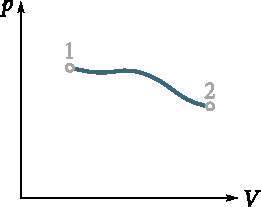
\includegraphics[scale=1.0]{figures/ch_10/fig_10_1.pdf}
		\caption[]{}
		\label{fig:10_1}
	\end{center}
\end{figure}

Mỗi \textbf{quá trình}, \ie, nghĩa là mỗi sự chuyển hệ từ trạng thái này sang trạng thái khác, gắn với sự phá hủy trạng thái cân bằng của hệ. Do đó, khi một quá trình nào đó tiến triển trong hệ, hệ sẽ liên tiếp đi qua các trạng thái không cân bằng. Trở lại quá trình vừa xét về sự nén khí trong bình được đậy bằng một pittông, có thể kết luận rằng là sự phá hủy trạng thái cân bằng khi đẩy pittông càng nhanh thì sự nén khí được thực hiện càng nhanh. Nếu đẩy pittông rất chậm thì sự cân bằng sẽ bị phá hủy không đáng kể và áp suất tại các điểm khác nhau sẽ khác một giá trị trung bình $p$ nào đó rất ít. Tại giới hạn, nếu sự nén khí xảy ra vô cùng chậm, thì tại mỗi điểm chất khí sẽ được đặc trưng bằng một giá trị xác định của áp suất. Do đó, trong trường hợp này trạng thái của chất khí tại mỗi thời điểm là trạng thái cân bằng và quá trình vô cùng chậm sẽ bao gồm sự nối tiếp các trạng thái cân bằng.

Một quá trình bao gồm sự nối tiếp liên tục các trạng thái cân bằng được gọi là \textbf{quá trình cân bằng} hoặc một \textbf{quá trình chuẩn tĩnh}. Từ điều đã nói suy ra rằng chỉ các quá trình vô cùng chậm mới có thể là quá trình cân bằng. Với sự tiến triển khá chậm, các quá trình thực có thể tiến tới quá trình cân bằng gần bao nhiêu cũng được.

Qúa trình cân bằng cũng có thể tiến triển theo hướng ngược lại thêm vào đó hệ đi qua cùng các trạng thái như trong quá trình thuận nhưng theo trình tự ngược lại. Do đó người ta cũng gọi các quá trình cân bằng là các \textbf{quá trình thuận nghịch}.

Qúa trình thuận nghịch (\ie, nghĩa là cân bằng) có thể được mô tả trên mặt phẳng tọa độ bằng một đường cong thích hợp (xem \fig{10_1}). Ta sẽ mô tả một cách quy ước các quá trình không thuận nghịch  (\ie, nghĩa là không cân bằng) bằng cách đường cong chấm chấm.

Qúa trình mà trong đó, sau một loạt các biến đổi, hệ lại trở về trạng thái ban đầu được gọi là một \textbf{quá trình tròn} hoặc một \textbf{chu trình}. Chu trình được mô tả trên đồ thị bằng một đường cong kín.

Các khái niệm về trạng thái không cân bằng và về quá trình thuận nghịch sẽ đóng vai trò lớn trong nhiệt động học. Tất cả các kết luận định lượng của nhiệt động học chỉ được áp dụng một cách thực sự vào các trạng thái cân bằng và vào các quá trình thuận nghịch.

\section{Nội năng của hệ}\label{sec:10_4}

Nội năng của một vật nào đó là năng lượng của vật đó trừ đi toàn bộ động năng của vật và thế năng của vật trong trường lực ngoài. Vậy, chẳng hạn, khi xác định nội năng của một khối lượng khí nào đó ta không cần tính năng lượng chuyển động của chất khí cùng với bình và năng lượng được gây bởi sự tồn tại của chất khí trong trường lực hấp dẫn của Trái Đất.

Do đó, động năng của chuyển động hỗn loạn của các phân tử, thế năng tương tác giữa các phân tử và năng lượng bên trong phân tử\footnote{Cần coi định nghĩa này như một định nghĩa bước đầu. Trong vật lý thống kê khái niệm nội năng sẽ được chính xác hóa. Tranh luận về sự chính xác hóa này đi ra ngoài giáo trình của vật lý đại cương} đều được đưa vào khái niệm nội năng.

Nội năng của một hệ vật là bằng tổng nội năng của mỗi vật riêng lẻ và năng lượng tương tác giữa các vật nghĩa là năng lượng tương tác giữa các phân tử trong một lớp mỏng tại biên giữa các vật. Năng lượng sau cùng này là rất nhỏ so với năng lượng của các vật vĩ mô tới mức có thể bỏ qua nó và coi nội năng của hệ các vật vĩ mô bằng tổng các nội năng của các vật tạo thành hệ. Vật nội năng là một đại lượng cộng tính.

Nội năng là một hàm trạng thái của hệ. Điều này có nghĩa là mỗi khi hệ ở trạng thái đã cho, nội năng của nó vốn có giá trị ở trạng thái này, không phụ thuộc vào tiền sử của hệ. Do đó, sự biến đổi nội năng khi chuyển từ hệ trạng thái này sang hệ trạng thái kia sẽ luôn luôn bằng hiệu các giá trị nội năng ở các trạng thái đó, không phụ thuộc vào đường đi theo đó thực hiện sự dịch chuyển, nghĩa là không phụ thuộc vào quá trình hoặc một loạt quá trình dẫn tới sự chuyển hệ từ trạng thái này tới trạng thái kia.

\section{Nguyên lý thứ nhất của nhiệt động học}\label{sec:10_5}

Nội năng có thể bị biến đổi chủ yếu là do hai quá trình khác nhau : Thực hiện công $A'$ trên vật và truyền cho vật nhiệt lượng $Q$. Sự thực hiện công kèm theo sự dịch chuyển các vật bên ngoài tác động lên hệ. Chẳng hạn, khi đẩy cái pít tông đậy một bình khí, pít tông dịch chuyển thực hiện một công $A'$ trên chất khí. Theo định luật 3 của Newton, khi đó chất khí thực hiện một công $A=-A'$ trên pit tông.

Sự truyền nhiệt cho chất khí không liên quan với sự dịch chuyển các vật bên ngoài và do đó không liên quan với sự thực hiện công vĩ mô (\ie, nghĩa là liên hệ với toàn bộ tập hợp các các phần tử tạo thành một vật) trên chất khí. Trong trường hợp này, sự thay đổi nội năng là do các phần tử riêng lẻ của vật được đốt nóng nhiều hơn thực hiện công trên các phần tử riêng lẻ của vật được đốt nóng ít hơn. Khi đó sự truyền năng lượng xảy ra qua sự bức xạ. Tập hợp các quá trình vi mô (\ie, nghĩa là các quá trình không phải toàn bộ vật mà chỉ các phần tử riêng lẻ của vật) dẫn tới sự truyền năng lượng từ vật này sang vật kia gọi là \textbf{sự truyển nhiệt}.

Tương tự như lượng năng lượng truyền từ vật này sang vật kia được xác định bằng công $A$ mà vật này thực hiện lên vật kia, lượng năng lượng truyền từ vật này sang vật kia bằng cách truyền nhiệt được xác định bằng \textbf{nhiệt lượng} $Q$ do vật này trao đổi cho vật kia. Vậy số gia nội năng của hệ phải bằng tổng công $A'$ được thực hiện trên hệ và nhiệt lượng $Q$ truyền cho hệ :
\begin{equation}\label{eq:10_6}
	U_2 - U_1 = Q + A'.
\end{equation}

\noindent
Ở đây $U_1$ và $U_2$ là các giá trị đầu và cuối của nội năng của hệ. Thường thay cho công $A'$ do các vật bên ngoài thực hiện trên hệ, người ta xét công $A$ (bằng $-A'$) do hệ thực hiện lên các vật bên ngoài. Đặt $-A$ thay cho $A'$ và giải phương trình \eqn{10_6} đối với $Q$, ta có : 
\begin{equation}\label{eq:10_7}
	Q = U_2 - U_1 + A.
\end{equation}

Phương trình~\eqref{eq:10_7} biểu diễn định luật bảo toàn năng lượng và là nội dung của \textbf{nguyên lý thứ nhất của nhiệt động học}. Có thể diễn đạt nó bằng lời như sau : \textit{nhiệt lượng truyền cho hệ làm tăng nội năng của hệ và làm cho hệ thực hiện công trên các vật bên ngoài}.

Nói như vật hoàn toàn không có nghĩa là khi truyền nhiệt, nội năng của hệ bao giờ cũng tăng. Có thể xảy ra là mặc dù truyền nhiệt cho hệ, năng lượng của nó không tăng mà lại giảm ($U_2<U_1$). Trong trường hợp này theo \eqn{10_7}, chúng ta có $A>Q$, \ie, nghĩa là hệ thực hiện công cả do nhiệt $Q$ nhận được và cả do lượng dự trữ nội năng mà độ giảm của nó bằng $U_1-U_2$. Cũng cần chú ý rằng các đại lượng $Q$ và $A$ trong \eqn{10_7} là các đại lượng đại số ($Q<0$ có nghĩa là thực tế hệ không nhận nhiệt mà là cho nhiệt).

Từ \eqn{10_7} suy ra rằng có thể đo nhiệt lượng $Q$ bằng các đơn vị giống như công và năng lượng. Trong hệ SI, jun được dùng làm đơn vị nhiệt lượng.

Một đơn vị đặc biệt được gọi là \textbf{calorie} cũng được dùng để đo nhiệt lượng. Một calorie bằng một nhiệt lượng cần thiết để đun nóng \SI{1}{\gram} nước từ \SIrange{19.5}{20.5}{\degreeCelsius}. Một kilocalorie bằng \SI{1000}{\calorie}.

Bằng cách thực nghiệm, chúng ta đã chứng minh được rằng 1 calorie bằng \SI{4.18}{\joule}. Do đó, một jun bằng \SI{0.24}{\calorie}. Đại lượng $E=\SI{4.18}{\joule\per\calorie}$ được gọi là \textbf{đương lượng cơ của nhiệt}.

Nếu các đại lượng trong \eqn{10_7} được biểu thị bằng các đơn vị khác nhau thì cần phải nhân một số đại lượng này với đương lượng tương ứng. Ví dụ, nếu chúng ta biểu thị $Q$ bằng calorie, $U$ và $A$ bằng jun, \eqn{10_7} sẽ được viết dưới dạng :
\begin{equation*}
	EQ = U_2 - U_1 + A
\end{equation*}

Dưới đây ta sẽ luôn giả thiết rằng $Q$, $A$ và $U$ được biểu thị bằng các đơn vị giống nhau và viết phương trình của nguyên lý thứ nhất của nhiệt động học dưới dạng \eqn{10_7}.

Khi tính công mà hệ thực hiện được hoặc nhiệt mà hệ nhận được thường phải chia quá trình được xét thành một dãy quá trình nguyên tố mà mỗi quá trình này ứng với một sự biến đổi rất nhỏ (nếu tại giới hạn là vô cùng nhỏ) các tham số của hệ. Phương trình \eqref{eq:10_7} đối với một quá trình nguyên tố có dạng:
\begin{equation}\label{eq:10_8}
	\Deltap{Q} = \Delta U + \Deltap{A}
\end{equation}

\noindent
Trong đó, $\Deltap{Q}$ là nhiệt lượng nguyên tố, $\Deltap{A}$ là công nguyên tố, và $\Delta U$ là số gia của nội năng của hệ trong tiến trình của quá trình nguyên tố đã cho.

Một chú ý rất quan trọng là không được coi $\Deltap{Q}$ và $\Deltap{A}$ như số gia của các đại lượng $Q$ và $A$. Có thể coi đại lượng $f$ nào đó ứng với một quá trình nguyên tố $\Delta$ như số gia của đại lượng này chỉ trong trường hợp nếu $\sum\Delta f$ ứng với sự dịch chuyển từ trạng thái này sang trạng thái khác không phụ thuộc vào quãng đường theo đó sự dịch chuyển thực hiện, nghĩa là đại lượng $f$ là một hàm trạng thái. Đối với hàm trạng thái có thể nói về "sự dự trữ" của nó tại mỗi trạng thái. Chẳng hạn, có thể nói về sự dự trữ nội năng mà hệ có tại các trạng thái khác nhau.

Ta sẽ thấy dưới đây, độ lớn của công mà hệ thực hiện và nhiệt lượng mà hệ nhận được đều phụ thuộc vào quãng đường dịch chuyển của hệ từ trạng thái này sang trạng thái kia. Do đó, cả $A$ và $Q$ đều không là các hàm trạng thái, vì thế không được nói về sự dự trữ nhiệt hoặc công mà hệ có tại các trạng thái khác nhau.

Như vậy, ký hiệu $\Delta$ đứng trước $A$ và $Q$ mang nghĩa khác so với khi đứng trước $U$. Để nhấn mạnh điều này, ký hiệu $\Delta$ trong trường hợp đầu được thêm dấu phẩy. Ký hiệu $\Delta U$ có nghĩa là số gia của nội năng, các ký hiệu $\Deltap{Q}$ và $\Deltap{A}$ không có nghĩa là số gia mà là lượng nhiệt và công nguyên tố.

Để biểu diễn phép tính, trong \eqn{10_8} người ta chuyển sang các vi phân. Khi đó phương trình của nguyên lý thứ nhất có dạng như sau :\footnote{In \eqn{10_9}, $\deriv{U}$ vi phân toàn phần, $\derivp{Q}$ và $\derivp{A}$ không là các vi phân toàn phần}
\begin{equation}\label{eq:10_9}
	\derivp{Q} = \deriv{U} + \derivp{A}.
\end{equation}

\noindent
Phép lấy tích phân \eqn{10_9} theo toàn bộ quá tình sẽ dẫn tới biểu thức :
\begin{equation*}
	Q = (U_2 - U_1) + A
\end{equation*}

\noindent
đồng nhất với phương trình \eqn{10_7}.

Chúng ta nhấn mạnh một lần nữa, ví dụ, không được phép viết kết quả  của phép lấy tích phân $\derivp{A}$ dưới dạng :
\begin{equation*}
	\int_{1}^{2} \derivp{A} = A_2 - A_1.
\end{equation*}

\noindent
Cách viết như vậy có nghĩa là công mà hệ thực hiện được là bằng hiệu các giá trị (\ie, nghĩa là các độ dự trữ) của công ở các dạng thứ hai và thứ nhất.

\section{Công do vật thực hiện khi biến đổi thể tích}\label{sec:10_6}

Có thể đặc trưng tương tác của một vật đã cho với các vật tiếp xúc với nó bằng áp suất mà vật tác dụng lên chúng. Nhờ áp suất có thể mô tả tương tác của chất khí với thành bình và cũng như các chất rắn hoặc chất lỏng với môi trường (chẳng hạn với chất khí) bao bọc quanh nó. Sự dịch chuyển các điểm đặt của các lực tương tác kéo theo sự biến đổi thể tích của vật. Do đó, công do vật này thực hiện trên các vật bên ngoài có thể được biểu thị qua áp suất và độ biến thiên thể tích của vật. Để tìm biểu thức này, ta xét ví dụ sau :

\begin{figure}[!htb]
	\begin{center}
		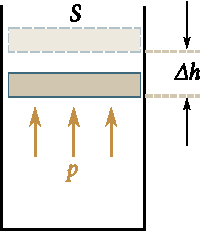
\includegraphics[scale=1.0]{figures/ch_10/fig_10_2.pdf}
		\caption[]{}
		\label{fig:10_2}
	\end{center}
\end{figure}

Giả sử chất khí chứa trong bình hình trụ được đậy khít bằng một pít tông có thể trượt dễ dàng (\fig{10_2}). Nếu do nguyên nhân nào đó chất khí bị dãn thì nó sẽ làm dịch chuyển pít tông. Công nguyên tố do chất khí thực hiện khi pít tông dịch chuyển một đoạn $\Delta h$ bằng:
\begin{equation*}
	\Deltap{A} = F \Delta h
\end{equation*}

\noindent
Trong đó, $F$ là lực mà chất khí tác dụng lên pít tông. Thay lực này bằng tích áp suất chất khí $p$ với diện tích pít tông $S$, ta có :
\begin{equation*}
	\Deltap{A} = p S \Delta h.
\end{equation*}

\noindent
Nhưng $S\Delta h$ là số gia của thể tích $\Delta V$. Do đó, có thể viết biểu thức đối với công nguyên tố như sau:
\begin{equation}\label{eq:10_10}
	\Deltap{A} = p\Delta V.
\end{equation}

Đại lượng $\Deltap{A}$ trong \eqn{10_10} rõ ràng là một đại lượng đại số. Thật vậy, khi nén khí các hướng của sự dịch chuyển $\Delta h$ và của lực $F$ mà chất khí tác dụng lên pít tông là ngược nhau. Do đó, công nguyên tố $\Deltap{A}$ sẽ âm. Số gia của thể tích $\Delta V$ trong trường hợp này cũng sẽ âm. Vậy công thức \eqn{10_10} cho một biểu thức đúng đối với công trong các biến đổi bất kỳ của thể tích chất khí.

Nếu áp suất chất khí vẫn không đổi (muốn vậy nhiệt độ phải được biến đổi đồng thời một cách thích hợp) thì công được thực hiện khi biến đổi thể tích từ giá trị $V_l$ đến $V_2$ sẽ bằng :
\begin{equation}\label{eq:10_11}
	A_{12} = p(V_2 - V_1).
\end{equation}

\noindent
Nếu như khi thể tích biến đổi áp suất cũng bị biến đổi thì công thức \eqn{10_10} chỉ đúng cho các  $\Delta V$ đủ nhỏ. Trong trường hợp này, công được thực hiện trong các biến đổi hữu hạn của thể tích phải được tính như tổng các nguyên tố dạng \eqn{10_10}, \ie, nghĩa là bằng cách lấy tích phân:
\begin{equation}\label{eq:10_12}
	A_{12} = \int_{V_1}^{V_2} p\,\deriv{V}.
\end{equation}

Các biểu thức tìm được đối với công là đúng trong các biến đổi bất kỳ của thể tích các chất rắn, lỏng và khí. Ở đây để thấy rõ ta hãy xét một ví dụ nữa. Ta lấy một vật rắn có hình dạng tùy ý được nhúng chìm vào môi trường này tác dụng lên vật một áp suất $p$ như nhau tại mọi điểm (\fig{10_3}). Ta giả sử rằng vật bị giãn nở sao cho các phần nguyên tố riêng biệt của bề mặt $\Delta S_i$ đều nhận được những độ dịch chuyển khác nhau $\Delta h_i$. Khi đó, phần thử $i$ thực hiện công $\Deltap{A}_i$ bằng $p\Delta S_i\Delta h_i$. Công do vật thực hiện có thể tìm được như tổng các công của các phần riêng lẻ:
\begin{equation*}
	\Deltap{A} = \sum_i\Deltap{A}_i = \sum_i p \Delta S_i \Delta h_i.
\end{equation*}

\begin{figure}[!htb]
	\begin{center}
		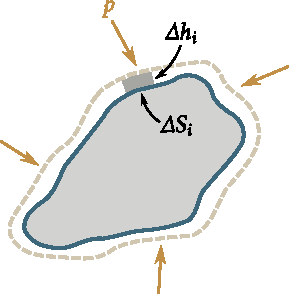
\includegraphics[scale=1.0]{figures/ch_10/fig_10_3.pdf}
		\caption[]{}
		\label{fig:10_3}
	\end{center}
\end{figure}

\noindent
Đưa $p$ giống nhau đối với tất cả các phần ra ngoài dấu tổng và chú ý rằng $\Delta S_i\Delta h_i$ cho số gia thể tích $\Delta V$ của vật, ta có thể viết $\Deltap{A}=p\Delta V$, nghĩa là ngay trong trường hợp tổng quát ta cũng đi tới \eqn{10_10}.

Ta hãy mô tả quá trình biến đổi thể tích của vật trên giản đồ $p$-$V$ (\fig{10_4}). Diện tích của dải được gạch hẹp trên đồ thị ứng với công nguyên tố $\Deltap{A}_i=p_i\Delta V_i$. Qúa rõ ràng rằng diện tích được giới hạn bởi trục $V$, đường cong $p=f(V)$, và các đường vuông góc dựng từ các điểm $V_1$ và $V_2$ về trị số bằng công được thực hiện khi biến đổi thể tích từ giá trị $V_1$ đến $V_2$. Công được thực hiện theo một quá trình hình tròn về trị số bằng diện tích được bao bởi đường cong (\fig{10_5}). Thật vậy, công ở phần $1$-$2$ là dương và về trị số bằng toàn bộ diện tích dưới đường cong, $\text{Area}_1+\text{Area}_2$ (ta xem xét một chu trình theo chiều kim đồng hồ). Công ở phần $2$-$1$ là âm và về trị số bằng diện tích không tô, $\text{Area}_2$. Vì thế, công trong một chu kỳ bằng số lượng với diện tích bao quanh bởi đường cong (khu vực được tô bóng, $\text{Area}_1$). Nó sẽ dương trong chu trình thuận (nghĩa là theo chiều kim đồng hồ), và âm trong chu trình nghịch.

Ta lưu ý rằng, sử dụng biểu thức (1.6.2) (với sự chuyển sang các vi phân) có thể viết phương trình (1.6.4) của nguyên lý thứ nhất của nhiệt động học như sau :
\begin{equation}\label{eq:10_13}
	\derivp{Q} = \deriv{U} + p\,\deriv{V}.
\end{equation}

\begin{figure}[!htb]
	\begin{minipage}[t]{0.5\linewidth}
		\begin{center}
			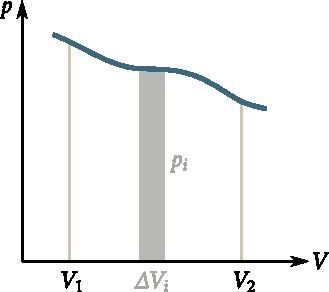
\includegraphics[scale=1.0]{figures/ch_10/fig_10_4.pdf}
			\caption[]{}
			\label{fig:10_4}
		\end{center}
	\end{minipage}
	\hspace{-0.0cm}
	\begin{minipage}[t]{0.5\linewidth}
		\begin{center}
			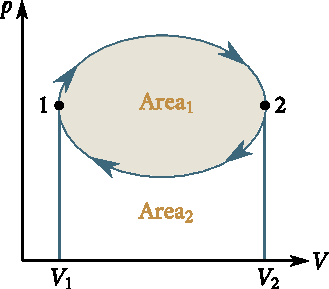
\includegraphics[scale=1.0]{figures/ch_10/fig_10_5.pdf}
			\caption[]{}
			\label{fig:10_5}
		\end{center}
	\end{minipage}
\end{figure}

\section{Nhiệt độ}\label{sec:10_7}

Có thể đi tới định nghĩa của khái niệm nhiệt độ trên cơ sở các suy nghĩ sau đây. Nếu các vật tiếp xúc nhau đều ở trạng thái cân bằng nhiệt, nghĩa là không trao đổi năng lượng với nhau bằng cách truyền nhiệt thì người ta gán cho các vật này nhiệt độ như nhau. Nếu khi thiết lập sự tiếp xúc nhiệt giữa các vật, một trong chúng truyền năng lượng cho vật khác bằng cách truyền nhiệt thì người ta gán cho vật thứ nhất một nhiệt độ lớn hơn vật thứ hai. Một loạt các tính chất của vật như thể tích, điện trở, v.v... phụ thuộc vào nhiệt độ. Bất kì tính chất nào trong các tính chất này có thể được sử dụng cho định nghĩa định lượng về nhiệt độ.
Ta hãy đưa một vài vật do ta chọn để đo nhiệt độ (vật nhiệt biểu) vào trạng thái cân bằng nhiệt với nước đá đang tan, trương trường hợp này ta gán nhiệt độ $0°$ cho vật và đặc trưng một cách định lượng tính chất đó của vật (mốc nhiệt độ) mà ta có ý định sử dụng nó để đo nhiệt độ. Giả sử ta chọn thể tích của vật làm một mốc như thế và giá trị của nó ở $0°$ là bằng $V_0$. Sau đó, ta hãy đưa chính vật đó vào trạng thái cân bằng nhiệt với nước sôi dưới áp suất khí quyển, ta hãy gán cho nó ở trạng thái này một giá trị nhiệt độ bằng $100°$ và ta hãy xác định thể tích $V_{100}$ tương ứng. Nếu thừa nhận là mốc nhiệt độ do ta chọn (trong ví dụ đang xét là thể tích) biến đổi tuyến tính với nhiệt độ thì ta phải gán nhiệt độ
\begin{equation}\label{eq:10_14}
	t = \frac{V - V_0}{V_{100} - V_0}\times 100\,\text{°}.
\end{equation}

\noindent
cho trạng thái mà trong đó vật nhiệt biểu có thể tích V. Thang nhiệt độ được thành lập bằng cách như vậy, như đã biết, được gọi là thang Celcius. Có thể viết hệ thức tương tự như (1.7.1) cho cả trường hợp khi để đo nhiệt độ người ta không lấy thể tích mà lấy một mốc nhiệt độ khác nào đó.

Nếu chia độ một nhiệt biểu bằng cách đã mô tả, có thể sử dụng nhiệt biểu để đo nhiệt độ bằng cách đưa nó vào trạng thái cân bằng nhiệt với vật có nhiệt độ mà ta quan tâm và tiến hành tính các độ lớn của thể tích.

Khi so sánh các nhiệt biểu sử dụng các vật nhiệt biểu khác nhau về tính chất (ví dụ thủy ngân, rượu, v.v...) hoặc các mốc nhiệt độ khác nhau (chẳng hạn thể tích và điện trở) người ta đã phát hiện ra là do cách chia độ bằng cách làm trùng nhau ở $0°$ và $100°$, các nhiệt biểu này sẽ không trùng nhau ở các nhiệt độ khác. Từ đây suy ra rằng để xác định. Nó được gọi là \textbf{thang nhiệt độ nhiệt động học}.

\textbf{Thang nhiệt độ thực hành quốc tế} năm 1968, hay còn được gọi là thang Celsius được sử dụng trong kỹ thuật và hàng ngày. Các nhà vật lý lại thấy \textbf{thang tuyệt đối} thuận tiện hơn cả. Nhiệt độ $T$ được tính theo thang này liên hệ với nhiệt độ $t$ theo thang Celcius bằng hệ thức :
\begin{equation*}
	T = t + 273.15.
\end{equation*}

\noindent
Người ta gọi đơn vị tuyệt đối là \textbf{Kelvin} (được ký hiệu là \si{\kelvin}). Trước đây người ta gọi nó là độ Kelvin (\si{\degree}K). Người ta đo nhiệt độ thực hành quốc tế bằng \textbf{độ Celsius} (\si{\degreeCelsius}). Giá trị của Kelvin và độ Celcius là như nhau. Nhiệt độ bằng \SI{0}{\kelvin} được gọi là  \textbf{không tuyệt đối}, và ứng với nó $t=\SI{-273.15}{\degreeCelsius}$.

Dưới đây ta sẽ chứng tỏ rằng nhiệt độ tuyệt đối tỉ lệ với động năng trung bình của chuyển động tịnh tiến các phân tử chất. Ý nghĩa vật lý của nhiệt độ tuyệt đối là ở đấy. 

\section{Phương trình trạng thái khí lý tưởng}\label{sec:10_8}

Trạng thái của một khối lượng khí đã cho được xác định bằng các giá trị của ba tham số : áp suất $p$, thể tích $V$, và nhiệt độ $T$. Các tham số này liên hệ với nhau một cách có quy luật, cho nên sự biến đổi các tham số khác. Sự liên hệ được chỉ ra có thể cho dưới dạng một hàm giải tích
\begin{equation}\label{eq:10_15}
	F(p,V,T) = 0.
\end{equation}

Hệ thức xác định sự liên hệ giữa các tham số của một vật nào đó được gọi là \textbf{phương trình trạng thái} của vật này. Do đó, \eqn{10_15} là phương trình trạng thái của khối lượng khí đã cho.

Chất khí mà sự tương tác giữa các phân tử là nhỏ không đáng kể có các tính chất đơn giản nhất. Chất khí như thế được gọi là \textbf{chất khí lý tưởng}. Sự tương tác giữa các phân tử của mọi chất khí trở nên yếu không đáng kể khi làm chân không cao, nghĩa là khi các mật độ khí nhỏ. Mỗi chất khí thực khi khá loãng có tính chất gần với khí lý tưởng. Một số chất khí như không khí, Nito, Oxy ngay cả ở các điều kiện bình thường, nghĩa là ở nhiệt độ phòng và áp suất khí quyển, cũng khác khí lý tưởng rất ít. Heli và Hydro có các tính chất đặc biệt gần với khí lý tưởng. 

Với các mật độ không lớn, các chất khí tuân theo phương trình:
\begin{equation}\label{eq:10_16}
	\frac{pV}{T} = \text{constant}.
\end{equation}

\noindent
với độ chính xác cao. Do đó, phương trình này được gọi là \textbf{phương trình trạng thái khí lý tưởng}.

Theo định luật do Avogadro (1776-1856) đã thiết lập thì các mol của mọi chất ở những điều kiện như nhau (nghĩa là cùng một nhiệt độ và áp suất) đều chiếm cùng một thể tích. Cụ thể là ở các điều kiện được gọi là \textbf{điều kiện tiêu chuẩn}, nghĩa là ở \SI{0}{\degreeCelsius} và áp suất bằng \SI{1}{\atm} (\SI{1.01e5}{\pascal}), thể tích của một mol chất khí bất kì $\SI{22.4}{\deci\metre\cubed\per\mole}=\SI{22.4e-3}{\metre\cubed\per\mole}$. Từ đó suy ra rằng trong trường hợp khi lượng khí bằng một mol, giá trị của hằng số trong \eqn{10_16} sẽ như nhau đối với tất cả chất khí. Bằng cách ký hiệu độ lớn của hằng số ứng với một mol bằng chữ $R$, chúng ta có thể viết \eqn{10_16} như sau:
\begin{equation}\label{eq:10_17}
	pV_{\text{m}} = RT.
\end{equation}

\noindent
Ta đặt ở $V$ chỉ số ``m'' để chứng tỏ rằng, nói về thể tích do một mol khí chiếm với $p$ và $T$ đã cho. Phương trình~\eqref{eq:10_17} là phương trình trạng thái của khí lý tưởng được viết cho một mol .

Đại lượng $R$ được gọi là \textbf{hằng số khí}. Theo \eqn{10_17} và định luật Avogadro,
\begin{equation*}
	R = \frac{pV_{\text{m}}}{T} = \frac{\num{1.01e5}\times\num{22.4e-3}}{273}\frac{\si{\pascal}\times\si{\metre\cubed\per\mol}}{\si{\kelvin}} = \SI{8.31}{\joule\per\mole\per\kelvin}.
\end{equation*}

\noindent
Đối với các tính toán thực tế, đôi khi người ta sử dụng giá trị $R$ tính ra lit-atmotphe trên mol-kenvin lại thuận tiện:
\begin{equation*}
	R = \frac{\SI{1}{\atm}\times\SI{22.4}{\liter\per\mole}}{\SI{273}{\kelvin}} = \SI{0.0820}{\liter\atm\per\mole\per\kelvin}.
\end{equation*}

Từ phương trình \eqn{10_17} đối với một mol dễ dàng chuyển sang phương trình đối với một khối lượng $m$ bất kỳ nếu chú ý rằng với cùng một áp suất và nhiệt độ, $\nu$ mol khí sẽ chiếm một thể tích lớn hơn một mol gấp $\nu$ lần: $V=\nu V_{\text{m}}$. Nhân \eqn{10_17} với $\nu=m/M$ (ở đây $m$ là khối lượng chất khí, $M$ là khối lượng phân tử gam) và thay thế $\nu V_{\text{m}}$ bởi $V$, ta có phương trình
\begin{equation}\label{eq:10_18}
	pV = \frac{m}{M}RT.
\end{equation}

\noindent
Phương trình này là phương trình trạng thái của khí lý tưởng được viết cho khối lượng $m$ của chất khí.

Phương trình~\eqref{eq:10_18} thêm một dạng khác. Muốn vậy ta đưa vào đại lượng
\begin{equation}\label{eq:10_19}
	k = \frac{R}{N_{\text{A}}}
\end{equation}

\noindent
($R$ là hằng số khí, $N_{\text{A}}$ là hằng số Avogadro). Đại lượng này được gọi là \textbf{hằng số Boltzmann}. Nó có ý nghĩa vật lý sâu xa hơn hằng số $R$. Trong Sec.~\ref{sec:11_5} sẽ chứng tỏ rằng $k$ là một hệ số tỉ lệ giữa năng lượng trung bình của chuyển động nhiệt của các phân tử và nhiệt độ tuyệt đối. Thay thế vào \eqn{10_19} các trị số của $R$ và $N_{\text{A}}$ ta được
\begin{equation*}
	k = \frac{\SI{8.31}{\joule\per\mole\per\kelvin}}{\SI{6.023e23}{\per\mole}} = \SI{1.38e-23}{\joule\per\kelvin}.
\end{equation*}

Nhân và chia vế phải của phương trình \eqn{10_18} cho $N_{\text{A}}$. Khi đó có thể viết phương trình dưới dạng
\begin{equation*}
	pV = \nu N_{\text{A}} k T.
\end{equation*}

\noindent
Tích $\nu N_{\text{A}}$ bằng số phân tử $N$ chứa trong khối lượng khí $m$. Nếu tính đến điều đó, ta sẽ thu được
\begin{equation}\label{eq:10_20}
	pV = NkT.
\end{equation}

Bây giờ ta chia cả 2 vế của phương trình \eqn{10_20} cho $V$. Chú ý rằng $N/V=n$ là số phân tử trong một đơn vị thể tích, ta đi tới công thức
\begin{equation}\label{eq:10_21}
	p = nkT.
\end{equation}

Các phương trình~\eqref{eq:10_18},~\eqref{eq:10_20}, và~\eqref{eq:10_21} là các dạng viết khác nhau của phương trình trạng thái khí lý tưởng.

The ratio of the mass of a gas to the volume it occupies gives the density of the gas: $p = m/V$. According to \eqn{10_18}, the density of an ideal gas is determined by the expression
\begin{equation}\label{eq:10_22}
	\rho = \frac{M p}{R T}.
\end{equation}

\noindent
Thus, the density of an ideal gas is proportional to the pressure and inversely proportional to the temperature.

The simple relation between the temperature and the remaining parameters of an ideal gas makes it tempting to use it as a thermometric substance. Ensuring a constant volume and using the pressure of the gas as the temperature feature, we can obtain a thermometer with an ideally linear temperature scale. In the following, we shall call this scale the \textbf{ideal gas temperature scale}.

In practice, according to an international agreement, hydrogen is taken as the thermometric body. The scale established for hydrogen with the use of \eqn{10_18} is called the \textbf{empirical temperature scale}.

\section{Internal Energy and Heat Capacity of an Ideal Gas}\label{sec:10_9}

Experiments show that the internal energy of an ideal gas depends only on the temperature:
\begin{equation}\label{eq:10_23}
	U = B T.
\end{equation}

\noindent
Here $B$ is a coefficient of proportionality that remains constant within quite a broad range of temperatures.

The failure of the internal energy to depend on the volume occupied by a gas indicates that the molecules of an ideal gas do not interact with one another the overwhelming part of the time. Indeed, if the molecules did interact with one another, the internal energy would contain as an addend the potential energy of interaction, and the latter would depend on the mean distance between the molecules, \ie, on $V^{1/3}$.

It must be noted that interaction should take place upon collisions, \ie, when the molecules come very close to one another. Such collisions are very few in number in a rarefied gas, however. Each molecule spends the predominating part of its time in free flight.

\textit{The heat capacity of a body is defined as the quantity equal to the amount of heat that must be imparted to the body to raise its temperature by one kelvin}. If the amount of heat $\derivp{Q}$ imparted to a body raises its temperature by $\deriv{T}$, then its heat capacity by definition is
\begin{equation}\label{eq:10_24}
	C_{\text{body}} = \frac{\derivp{Q}}{\deriv{T}}.
\end{equation}

\noindent
This quantity is measured in joules per kelvin (\si{\joule\per\kelvin}).

We shall denote the capacity of a mole of a substance, called the \textbf{molar heat capacity}, by the symbol $C$. It is measured in joules per mole-kelvin (\si{\joule\per\mole\per\kelvin}).

The heat capacity of a unit mass of a substance is called the \textbf{specific heat capacity}. We shall use the symbol $c$ for it. The quantity $c$ is measured in joules per kilogramme-kelvin (\si{\joule\per\kilo\gram\per\kelvin}).

The following relation obviously holds between the heat capacity of a mole of a substance and the specific heat capacity of the same substance:
\begin{equation}\label{eq:10_25}
	c = \frac{C}{M}
\end{equation}

\noindent
($M$ is the molar mass).

The value of the heat capacity depends on the conditions in which a body is heated. The heat capacity for heating at a constant volume or a constant pressure is of the greatest interest. The heat capacities at constant volume and constant pressure are designated by $C_V$ and $C_p$, respectively.

When heating occurs at constant volume, a body does no work on external bodies, and, consequently, according to the first law of thermodynamics [see Eq. \eqref{eq:10_9}], all the heat is spent on the increment of the internal energy of the body:
\begin{equation}\label{eq:10_26}
	\derivp{Q}_V = \deriv{U}.
\end{equation}

\noindent
It can be seen from \eqn{10_26} that the heat capacity of any body at constant volume is
\begin{equation}\label{eq:10_27}
	C_V = \left(\diffpartial{U}{T}\right)_V.
\end{equation}

\noindent
This notation stresses the fact that when differentiating the expression for $U$ with respect to $T$, the volume must be considered constant. For an ideal gas, $U$ depends only on $T$, and \eqn{10_27} can be written in the form
\begin{equation*}
	C_V = \diff{\ab{U}{m}}{T}
\end{equation*}

\noindent
(to obtain the molar heat capacity of a gas, we must take the internal energy of a mole).

Equation~\eqref{eq:10_23} for one mole of a gas has the form $\ab{U}{m}=\ab{B}{m}T$. Differentiating it with respect to $T$, we find that $C_V=\ab{B}{m}$. Thus, the expression for the internal energy of one mole of an ideal gas can be written in the form
\begin{equation}\label{eq:10_28}
	\ab{U}{m} = C_V T
\end{equation}

\noindent
where $C_V$ is a constant quantity---the molar heat capacity of a gas at constant volume.

The internal energy of an arbitrary mass $m$ of a gas will equal the internal energy of one mole multiplied by the number of moles of the gas in the mass $m$:
\begin{equation}\label{eq:10_29}
	U = \frac{m}{M}C_V T.
\end{equation}

If a gas is heated at constant pressure, it will expand, doing positive work on external bodies. Consequently, more heat will be needed to raise the temperature of the gas by one kelvin in this case than when heating it at constant volume---part of the heat will be used by the gas to do work. Hence, the heat capacity at constant pressure must be greater than that at constant volume.

Let us write \eqn{10_13} of the first law of thermodynamics for a mole of a gas:
\begin{equation}\label{eq:10_30}
	\derivp{Q}_p = \deriv{\ab{U}{m}} + p\,\deriv{\ab{V}{m}}.
\end{equation}

\noindent
The subscript $p$ of $\derivp{Q}$ in this expression indicates that heat is imparted to the gas in conditions when $p$ is constant. Dividing \eqn{10_30} by $\deriv{T}$, we get an expression for the molar heat capacity of a gas at constant pressure:
\begin{equation}\label{eq:10_31}
	C_p = \diff{\ab{U}{m}}{T} + p\left(\diffpartial{\ab{V}{m}}{T}\right)_p.
\end{equation}

\noindent
The addend $\diffin{\ab{U}{m}}{T}$ equals, as we have seen, the molar heat capacity of a gas at constant volume. Therefore, \eqn{10_31} can be written as follows:
\begin{equation}\label{eq:10_32}
	C_p = C_v + p\left(\diffpartial{\ab{V}{m}}{T}\right)_p.
\end{equation}

The quantity $\left(\diffinpartial{\ab{V}{m}}{T}\right)_p$ is the increment of the volume of a mole when the temperature is raised by one kelvin obtained with $p$ being constant. According to the equation of state~\eqref{eq:10_17}, we have $\ab{V}{m}=RT/p$. Differentiating this expression with respect to $T$ provided that $p=\text{constant}$, we find
\begin{equation*}
	\left(\diffpartial{\ab{V}{m}}{T}\right)_p = \frac{R}{p}.
\end{equation*}

\noindent
Finally, using this result in \eqn{10_32}, we get
\begin{equation}\label{eq:10_33}
	C_p = C_v + R.
\end{equation}

Thus, the work done by a mole of an ideal gas when its temperature is raised by one kelvin at constant pressure equals the molar gas constant. It must be noted that \eqn{10_33} has been obtained by using an equation of state for an ideal gas and, consequently, holds only for an ideal gas.

The quantity
\begin{equation}\label{eq:10_34}
	\gamma = \frac{C_p}{C_V}
\end{equation}

\noindent
is a quantity characterizing every gas. For monatomic gases, its value is close to $1.67$, for biatomic gases to $1.4$, for triatomic gases to $1.33$, etc. In the following (see Sec.~\ref{sec:11_5}), we shall see that the value of $\gamma$ is determined by the number and the nature of the degrees of freedom of the molecule.

Substituting for $C_p$ in \eqn{10_34} its value from \eqn{10_33}, we have
\begin{equation*}
	\gamma = \frac{C_V + R}{C_V} = 1 + \frac{R}{C_V}
\end{equation*}

\noindent
whence
\begin{equation}\label{eq:10_35}
	C_V = \frac{R}{1 - \gamma}.
\end{equation}

\noindent
Using this value of $C_V$ in \eqn{10_29}, we get the following expression:
\begin{equation}\label{eq:10_36}
	U = \frac{m}{M}\left(\frac{RT}{\gamma - 1}\right).
\end{equation}

\noindent
Comparison with \eqn{10_18} gives still another expression for the internal energy of an ideal gas:
\begin{equation}\label{eq:10_37}
	U = \left(\frac{1}{\gamma - 1}\right) pV.
\end{equation}

\section{Equation of Adiabat of an Ideal Gas}\label{sec:10_10}

In the course of a process, a gas, in addition to an equation of state, obeys another condition determined by the nature of the process. For example, the condition $p=\text{constant}$ is observed in the so-called \textbf{isobaric process}. The condition $V=\text{constant}$ holds in an \textbf{isochoric process}. Finally, in an \textbf{isothermal process}, $T=\text{constant}$. For an ideal gas, the condition $T=\text{constant}$ is equivalent to the condition
\begin{equation}\label{eq:10_38}
	pV = \text{constant}.
\end{equation}

\noindent
Equation~\eqref{eq:10_38} is called the equation of an isotherm of an ideal gas, and the curve determined by this equation is named an \textbf{isotherm}.

\textit{A process going on without heat exchange with the surroundings} is called \textbf{adiabatic}. Let us find an equation relating the parameters of an ideal gas in an adiabatic process. Introducing \eqn{10_29} for $\deriv{U}$ of an ideal gas into \eqn{10_13} of the first law of thermodynamics, we obtain
\begin{equation*}
	\derivp{Q} = \frac{m}{M}C_V\,\deriv{T} + p\,\deriv{V}.
\end{equation*}

\noindent
Since for an adiabatic process we have $\derivp{Q}=0$, the following condition must be observed:
\begin{equation}\label{eq:10_39}
	\frac{m}{M}C_V\,\deriv{T} + p\,\deriv{V} = 0.
\end{equation}

Now let us express $p$ through $V$ and $T$ in accordance with the equation of state for an ideal gas~\eqref{eq:10_18}:
\begin{equation*}
	p = \frac{m}{M}\frac{RT}{V}
\end{equation*}

\noindent
and introduce this expression into \eqn{10_39}. As a result, after cancelling the factor $m/M$ differing from zero, we get
\begin{equation*}
	C_V\,\deriv{T} + RT\,\frac{\deriv{V}}{V} = 0.
\end{equation*}

\noindent
Let us transform the above expression as follows:
\begin{equation*}
	\frac{\deriv{T}}{T} + \frac{R}{C_V}\,\frac{\deriv{V}}{V} = 0.
\end{equation*}

\noindent
This expression can be written in the form
\begin{equation*}
	\upd\left(\ln{T} + \frac{R}{C_V}\,\ln{V}\right) = 0
\end{equation*}

\noindent
whence it follows that in an adiabatic process
\begin{equation}\label{eq:10_40}
	\ln{T} + \frac{R}{C_V}\,\ln{V} = \text{constant}.
\end{equation}

In accordance with \eqn{10_35}, the ratio $R/C_V$ can be replaced withy $\gamma - 1$, where $\gamma=C_p/C_V$. Making this substitution in \eqn{10_40} and converting to a power, we get
\begin{equation}\label{eq:10_41}
	T V^{\gamma - 1} = \text{constant}.
\end{equation}

This equation is an equation of an adiabat of an ideal gas in variable $T$ and $V$. We can pass over from this equation to one in variable $p$ and $V$ by replacing $T$ in it with $p$ and $V$ in accordance with the equation of state for an ideal gas~\eqref{eq:10_18}:
\begin{equation*}
	T = \frac{M}{m}\frac{pV}{R}.
\end{equation*}

\noindent
Using this expression in \eqn{10_41} and taking into account that $m$, $M$ and $R$ are constants, we get
\begin{equation}\label{eq:10_42}
	p V^{\gamma} = \text{constant}.
\end{equation}

\noindent
[The values of the constants in Eqs.~\eqref{eq:10_40}-\eqref{eq:10_42} are obviously
different.]

Expression~\eqref{eq:10_42} is an equation of an adiabat of an ideal gas in variable $p$ and $V$. It is also called the \textbf{Poisson equation}.

\begin{figure}[!htb]
	\begin{center}
		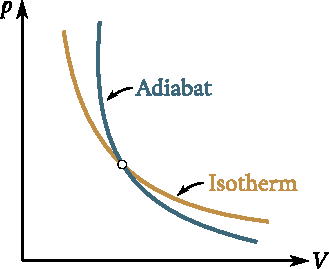
\includegraphics[scale=1.0]{figures/ch_10/fig_10_6.pdf}
		\caption[]{}
		\label{fig:10_6}
	\end{center}
\end{figure}

It follows from a comparison of the adiabat equation~\eqref{eq:10_42} with the isotherm equation~\eqref{eq:10_38} that an adiabat is steeper than an isotherm. Let us calculate $\diffin{p}{V}$ for an isotherm and an adiabat at the same point with the coordinates $p$ and $V$ (\fig{10_6}). Differentiation of \eqn{10_38} yields
\begin{equation*}
	p\,\deriv{V} + V\,\deriv{p} = 0
\end{equation*}

\noindent
whence for an isotherm we obtain
\begin{equation}\label{eq:10_43}
	\diff{p}{V} = -\frac{p}{V}.
\end{equation}

\noindent
Differentiation of Eq. (10.42) yields
\begin{equation*}
	p \gamma V^{\gamma - 1}\,\deriv{V} + V^{\gamma}\,\deriv{p} = 0
\end{equation*}

\noindent
whence
\begin{equation*}
	\diff{p}{V} = -\gamma \frac{p}{V}.
\end{equation*}

\noindent
Thus, the slope of an adiabat is $\gamma$ times greater than that of an isotherm.

We assumed in all our reasoning that the state of a gas at each moment is characterized by definite values of the parameters $p$ and $T$, \ie, in other words, that the adiabatic process being considered is reversible. We know that only a very slow process can be reversible. At the same time, since nature knows of no substances that do not conduct heat absolutely, the amount of heat exchanged by a system with its surroundings will be the smaller, the shorter is the time taken by a process.

Thus, only fast processes can be close to an adiabatic one. An example of such a process are the compression and expansion occurring at each point of a gas in which a sound wave is propagating. Notwithstanding the fact that within the confines of a large volume the state of the gas is not an equilibrium one ($p$ and $T$ are different at different points), the behaviour of the gas within the limits of each sufficiently small volume is quite satisfactorily described by \eqn{10_42} of an adiabat.

\section{Polytropic Processes}\label{sec:10_11}

\textit{Processes in which the heat capacity of a body remains constant} are defined as \textbf{polytropic} ones. Thus, the condition which is observed in a polytropic process is
\begin{equation}\label{eq:10_44}
	C = \text{constant}.
\end{equation}

Let us find the equation of a polytrope for an ideal gas. We shall write equation~\eqref{eq:10_13} of the first law for one mole of gas, substituting $C\,\deriv{T}$ for $\derivp{Q}$ and $C_V\,\deriv{T}$ for $\deriv{U}$:
\begin{equation}\label{eq:10_45}
	C\,\deriv{T} = C_V\,\deriv{T} + p\,\deriv{V}.
\end{equation}

\noindent
This equation includes all three parameters: $p$, $V$ and $T$. One of them can be excluded with the aid of an equation of state. To obtain an equation of a polytrope directly in variable $p$ and $V$, let us exclude $T$. For this end, let us differentiate the equation $pV=RT$:
\begin{equation}\label{eq:10_46}
	p\,\deriv{V} + V\,\deriv{p} = R\,\deriv{T} + .
\end{equation}

\noindent
Excluding $\deriv{T}$ from Eqs.~\eqref{eq:10_45} and~\eqref{eq:10_46} and bringing together similar terms, we get
\begin{equation}\label{eq:10_47}
	(C - C_V - R) p\,\deriv{V} + (C - C_V) V\,\deriv{p} = 0.
\end{equation}

\noindent
Substituting $C_p$ for $C_V+R$ [see \eqn{10_33}] and dividing \eqn{10_47} by $pV$, we arrive at the differential equation
\begin{equation}\label{eq:10_48}
	(C - C_p)\,\frac{\deriv{V}}{V} + (C - C_V) \,\frac{\deriv{p}}{p} = 0.
\end{equation}

The quantities $C$, $C_p$, and $C_V$ are constants. Therefore, integration of \eqn{10_48} gives the expression
\begin{equation}\label{eq:10_49}
	(C - C_p)\,\ln{V} + (C - C_V)\,\ln{p} = \text{constant}.
\end{equation}

\noindent
Dividing this expression by $C-C_V$ (which is possible if $C\neq C_v$) and converting to a power, we get
\begin{equation}\label{eq:10_50}
	pV^n = \text{constant}
\end{equation}

\noindent
where
\begin{equation}\label{eq:10_51}
	n = \frac{C - C_p}{C - C_V}.
\end{equation}

It is exactly \eqn{10_50} that is the required equation of a polytrope of an ideal gas for $C\neq C_v$. The quantity $n$ determined by \eqn{10_51} is called the \textbf{polytropic exponent} or \textbf{index}.

Let us turn to \eqn{10_49} to establish the nature of a polytropic process when $C=C_V$. For this condition, the equation acquires the form $(C-C_p)\ln{V}=\text{constant}$, whence it follows that $V$ in the course of the process remains constant. Hence, a polytropic process with $C=C_V$ is an isochoric one. This could be foreseen because $C_V=\text{constant}$ and is the heat capacity at constant volume, \ie, in	an isochoric process. By \eqn{10_51}, the polytropic exponent in an isochoric process equals infinity.

The other processes treated in the preceding section also relate to the category of polytropic processes. For an isobaric process, we have $n=0$ [see \eqn{10_50}], for an isothermal one $n=1$, and, finally, for an adiabatic process $n=\gamma$. The value of the polytropic exponent $n$ for these processes are given in Table~\ref{table:10_1}.

\begin{table}[!htb]
	\renewcommand{\arraystretch}{1.2}
	\caption{ }
	\vspace{-0.6cm}
	\label{table:10_1}
	\begin{center}\resizebox{0.233\linewidth}{!}{
			\begin{tabular}{lc}
				\toprule[1pt]
				\textbf{Process} & $n$\\
				\midrule[0.5pt]\midrule[0.5pt]
				Isobaric & 0\\
				Isothermal & 1\\
				Adiabatic & $\gamma$\\
				Isochoric & $\infty$\\
				\bottomrule[1pt]
			\end{tabular}
	}\end{center}
\end{table}

Solving \eqn{10_51} relative to $C$, we get an equation for the heat capacity of an ideal gas in a polytropic process:
\begin{equation}\label{eq:10_52}
	C = \frac{n C_V - C_p}{n - 1}.
\end{equation}

\noindent
The introduction of $n=\gamma$ causes \eqn{10_52} to become equal to zero [\eqn{10_35} must be taken into account in verifying this statement]. Consequently, the heat capacity of an ideal gas in an adiabatic process equals zero. The heat capacity of all bodies vanishes in an adiabatic process. This can be seen from the fact that in an adiabatic process $\derivp{Q}=0$, whereas $\deriv{T}$ differs from zero.

The introduction of $n=1$ causes \eqn{10_52} to equal infinity. Thus, in an isothermal process, the heat capacity is infinitely great. The explanation is that in an isothermal process $\deriv{T}=0$, whereas $\derivp{Q}$ differs from zero.

\section{Work of an Ideal Gas in Different Processes}\label{sec:10_12}

The work done by a body on external bodies when it passes from state $1$ to state $2$ is
\begin{equation}\label{eq:10_53}
	A_{12} = \int_{V_1}^{V_2} p\,\deriv{V}
\end{equation}

\noindent
[see \eqn{10_12}]. To perform integration, we must express $p$ through $V$. For this purpose, we shall use the relation between $p$ and $V$ in different processes.

Equation~\eqref{eq:10_50} of a polytrope of an ideal gas can be written as follows:
\begin{equation*}
	pV^n = p_1V_1^n = p_2V_2^n
\end{equation*}

\noindent
where $ p_1, V_1$ and $ p_2, V_2$ are the values of the pressure and volume of the gas in the first (initial) and second (final) states, respectively, and $p$ and $V$ are the pressure and volume in any intermediate state. The above equation allows us to express the pressure of a gas through its volume and the values of the parameters in the initial or final state. Taking the former, we have
\begin{equation*}
	p = \frac{p_1V_1^n}{V^n}.
\end{equation*}

\noindent
Introduction of this equation into \eqn{10_53} yields
\begin{equation}\label{eq:10_54}
	A_{12} = p_1 V_1^n\, \int_{V_1}^{V_2} \frac{\deriv{V}}{V^n}.
\end{equation}

\noindent
Let us first consider the case when $n\neq 1$; the integral in \eqn{10_54} for it is
\begin{equation*}
	\int_{V_1}^{V_2} \frac{\deriv{V}}{V^n} = \left(\frac{1}{n-1}\right) \left(\frac{1}{V_1^{n-1}} - \frac{1}{V_2^{n-1}}\right).
\end{equation*}

\noindent
Using this value of the integral in \eqn{10_54} and performing simple transformations, we get
\begin{equation}\label{eq:10_55}
	A_{12} = \frac{p_1 V_1}{n-1} \left[1 - \left(\frac{V_1}{V_2}\right)^{n-1} \right].
\end{equation}

This equation can be transformed by taking advantage of the fact that no matter what process occurs with an ideal gas, its parameters are related by an equation of state. In particular, this also holds for the initial state:
\begin{equation}\label{eq:10_56}
	p_1 V_1 = \frac{m}{M}RT_1.
\end{equation}

\noindent
Taking \eqn{10_56} into account, we can write \eqn{10_55} in the form
\begin{equation}\label{eq:10_57}
	A_{12} = \frac{m}{M} \left(\frac{RT_1}{n-1}\right) \left[1 - \left(\frac{V_1}{V_2}\right)^{n-1} \right].
\end{equation}

Equations~\eqref{eq:10_55} and~\eqref{eq:10_57} give the work done by an ideal gas in any polytropic process except for an isothermal one [which corresponds to $n=1$. In this case, Eqs.~\eqref{eq:10_55} and~\eqref{eq:10_57} become indefinite]. In particular, for an adiabatic process
\begin{equation}\label{eq:10_58}
	A_{12} = \left(\frac{p_1 V_1}{\gamma - 1}\right) \left[1 - \left(\frac{V_1}{V_2}\right)^{n-1} \right]
\end{equation}

\noindent
or
\begin{equation}\label{eq:10_59}
	A_{12} = \frac{m}{M} \left(\frac{RT_1}{\gamma - 1}\right) \left[1 - \left(\frac{V_1}{V_2}\right)^{n-1} \right].
\end{equation}

To calculate the work of an ideal gas in an isothermal process, let us express the pressure in \eqn{10_53} through other quantities in accordance with an equation of state. The result is (we can put $T$ outside the integral since it is constant):
\begin{equation*}
	A_{12} = \frac{m}{M}RT\, \int_{V_1}^{V_2} \frac{\deriv{V}}{V} = \frac{m}{M} RT\,\ln\left(\frac{V_2}{V_1}\right).
\end{equation*}

\noindent
Thus, the work done by an ideal gas in an isothermal process is
\begin{equation}\label{eq:10_60}
	A_{12} = \frac{m}{M} RT\,\ln\left(\frac{V_2}{V_1}\right).
\end{equation}

In an isobaric process, the work done by any body including an ideal gas, as can be seen from \eqn{10_53}, is
\begin{equation}\label{eq:10_61}
	A_{12} = p(V_2 - V_1).
\end{equation}

\noindent
The same result is obtained if we assume that $n=0$ in \eqn{10_55}. We shall note in concluding that the work equals zero in an isochoric process. This holds for any bodies.

\section{Van der Waals Gas}\label{sec:10_13}

We mentioned in Sec.~\ref{sec:10_8} that the behaviour of real gases is well described by \eqn{10_17}, \ie,
\begin{equation*}
	p\ab{V}{m} = RT
\end{equation*}

\noindent
only at low densities, \ie, at not too high pressures and sufficiently high temperatures [see \eqn{10_22}]. Considerable deviations from this equation are observed with an increase in the pressure and a decrease in the temperature. The second column of Table~\ref{table:10_2} gives the values of the product $pV$ for the mass of nitrogen occupying a volume of one litre in standard conditions. These values are given for different pressures and the same temperature \SI{0}{\degreeCelsius}.

\begin{table}[!htb]
	\vspace{-0.2cm}
	\renewcommand{\arraystretch}{1.2}
	\caption{ }
	\vspace{-0.6cm}
	\label{table:10_2}
	\begin{center}\resizebox{0.6\linewidth}{!}{
			\begin{tabular}{ccc}
				\toprule[1pt]
				$p$, [\si{\atm}] & $pV$, [\si{\atm\liter}] & $\left(p+\dfrac{a'}{V^2}\right)(V-b')$, [\si{\atm\liter}]\\
				\midrule[0.5pt]\midrule[0.5pt]
				$1$ 	& 	$1.000$ 	&	$1.000$\\
				$100$ 	&	$0.994$		&	$1.000$\\
				$200$	&	$1.048$		&	$1.009$\\
				$500$	&	$1.390$		&	$1.014$\\
				$1000$	&	$2.069$		&	$0.893$\\
				\bottomrule[1pt]
			\end{tabular}
	}\end{center}
\end{table}

According to \eqn{10_17}, the product $pV$ must remain constant when the temperature does not change. Actually, as can be seen from the table, appreciable deviations are observed at a pressure of about \SI{200}{\atm}. They grow continuously with increasing pressure and reach over $100$\% at \SI{1000}{\atm}. These deviations are not surprising because when the density grows, the volume of the molecules and the interaction between them begin to play a greater and greater part.

A great variety of equations were proposed to describe the behaviour of gases within a broad density range. The one proposed by J. van der Waals is the simplest of them, while giving sufficiently good results. This equation was obtained by introducing corrections into \eqn{10_17} and has the following form:
\begin{equation}\label{eq:10_62}
	\left(p+\frac{a}{\ab{V}{m}^2}\right)(\ab{V}{m} - b) = RT
\end{equation}

\noindent
where $p$ is the pressure exerted on the gas from outside (equal to the pressure of the gas on the walls of the vessel it occupies), and $a$ and $b$ are van der Waals constants. Their values differ for different gases and are determined experimentally. If the pressure is measured in pascals and the volume in cubic metres per mole, then the constant $a$ is in \si{\pascal~\metre^6~\mole^{-1}}, and the constant $b$ is in \si{\metre\cubed\per\mole}. Sometimes the constants $a$ and $b$ are expressed in \si{\atm\liter\squared} and \si{\liter\per\mole}, respectively.

Owing to the mutual attraction between its molecules, a gas, as it were, is compressed by a greater pressure than the pressure $p$ exerted on it by the walls of the vessel confining it. The correction $a/\ab{V}{m}^2$ characterizes the addition to the external pressure due to the mutual attraction of the molecules. Molecules have an appreciable action on one another within the limits of small distances called the \textbf{radius of molecular action}. The force of mutual attraction of two elementary volumes having dimensions of the order of this radius is proportional both to the number of molecules contained in one of the volumes and to that in the other volume. Each of these numbers, in turn, is proportional to the number of molecules in unit volume, \ie, is inversely proportional to the volume of the gas. These considerations can be used to explain the circumstance that the correction to the pressure in \eqn{10_62} has the form $a/\ab{V}{m}^2$.

Since the molecules have a finite volume, the space available for motion of the molecules is less than the volume of the vessel $\ab{V}{m}$ The correction $b$ in \eqn{10_62} characterizes the part of the volume that is not available for motion of the molecules. In its order of magnitude, it equals several total volumes of the molecules contained in a mole of a gas.

Equation~\eqref{eq:10_62} has been written for one mole of a gas. To go over to an equation for an arbitrary mass $m$, we must take into account that $\nu$ moles of a gas in the same conditions occupy a volume that is $\nu$ times greater: $V=\nu\ab{V}{m}.$ Substituting $V/\nu$ for $\ab{V}{m}$ in \eqn{10_62}, we get
\begin{equation*}
	\left(p + \frac{\nu^2 a}{V^2}\right) \left(\frac{V}{\nu} - b\right) = RT.
\end{equation*}

\noindent
Multiplying this equation by $\nu$ and introducing the symbols
\begin{equation}\label{eq:10_63}
	a' = \nu^2 a,\quad b' = \nu b
\end{equation}

\noindent
we arrive at the van der Waals equation for $\nu$ moles:
\begin{equation}\label{eq:10_64}
	\left(p + \frac{a'}{V^2}\right) (V - b') = \nu RT.
\end{equation}

\noindent
The symbols $a'$ and $b'$ designate the van der Waals constants for $\nu$ moles. Equations~\eqref{eq:10_63} show how they are related to $a$ and $b$. The constant $a'$ is measured in \si{\pascal~\metre^6}, and $b'$ in \si{\metre\cubed}.

How much better the van der Waals equation shows the behaviour of gases than \eqn{10_17} can be seen from the data contained in Table~\ref{table:10_2}. The third column of the table gives the values of the quantity $(p+a'/V^2)(V-b')$, which ought to be constant according to \eqn{10_64}, for the same mass of nitrogen for which the values of $pV$ are given in the second column. Inspection of the table shows that the van der Waals equation agrees much better with experimental data than \eqn{10_17}.

Since all real gases approach ideal gases in their properties when their density diminishes, the van der Waals equation in the limit, when the volume tends to infinity, transforms into \eqn{10_17}. We can convince ourselves that this is true by factoring out $p$ and $V$ in \eqn{10_64}:
\begin{equation*}
	pV\left(1 + \frac{1}{pV}\frac{a'}{V}\right)\left(1 - \frac{b'}{V}\right) = \nu RT
\end{equation*}

\noindent
and taking into consideration that the product $pV$ is approximately constant.

Real gases obey the van der Waals equation only approximately. An imaginary gas that obeys \eqn{10_62} exactly is called a van der Waals gas.

The internal energy of a van der Waals gas must include, in addition to the kinetic energy of the molecules, the energy of interaction between them. To find the internal energy of a van der Waals gas, let us take advantage of the circumstance that the work done in the expansion of a gas against the forces of mutual attraction of the molecules to one another equals the increment of the interaction energy: $\derivp{A}= \deriv{\ab{E}{p}}$. The forces of mutual attraction between the molecules are taken into account in \eqn{10_62} with the aid of the addition $a/\ab{V}{m}^2$ to the pressure. Accordingly, the work against the forces of interaction between the molecules can be represented in the form $(a/\ab{V}{m}^2)\,\deriv{\ab{V}{m}}$ (similarly, the work done by a gas against the external forces is determined by the expression $p\,\deriv{V}$). Thus,
\begin{equation*}
	\deriv{\ab{E}{p}} = \frac{a}{\ab{V}{m}^2}\,\deriv{\ab{V}{m}}.
\end{equation*}

\noindent
Integration of this expression shows that
\begin{equation}\label{eq:10_65}
	\ab{E}{p} = -\frac{a}{\ab{V}{m}} + \text{constant}.
\end{equation}

The internal energy of a van der Waals gas depends on both the volume and the temperature. Hence, the expression for $U$ has the form
\begin{equation*}
	U = f(T) - \frac{a}{\ab{V}{m}}
\end{equation*}

\noindent
[we have included the constant of \eqn{10_65} in $f(T)$]. This expression in the limit, when the volume tends to infinity, must transform into \eqn{10_28} for the internal energy of an ideal gas. Therefore, $f(T)=C_VT$.

Thus, the internal energy of a mole of a van der Waals gas is determined by the equation
\begin{equation}\label{eq:10_66}
	\ab{U}{m} = C_VT - \frac{a}{\ab{V}{m}}.
\end{equation}

\noindent
The internal energy of $\nu$ moles will be $\nu$ times greater:
\begin{equation}\label{eq:10_67}
	U = \nu C_VT - \frac{a'}{V}
\end{equation}

\noindent
(we have taken into consideration that $\nu^2a=a'$ and $\nu\ab{V}{m}=V$). By Eqs.~\eqref{eq:10_66} and~\eqref{eq:10_67}, we can find the approximate values of the internal energy of real gases.

\section{The Barometric Formula}\label{sec:10_14}

The atmospheric pressure at the altitude $h$ is due to the weight of the layers of gas above this altitude. Let $p$ be the pressure at the altitude $h$. Hence, the pressure at the altitude $h+\deriv{h}$ will be $p+\deriv{p}$. If $\deriv{h}$ is greater than zero, then $\deriv{p}$ will be less than zero because the weight of the higher layers of the atmosphere and, therefore, the pressure, diminish with the altitude. The difference between the pressures $p$ and $p+\deriv{p}$ equals the weight of the gas contained in the volume of a cylinder with a base area of unity and an altitude of $\deriv{h}$ (\fig{10_7}):
\begin{equation*}
	p - (p + \deriv{p}) = \rho g\,\deriv{h}
\end{equation*}

\noindent
where $\rho$ is the density of the gas at the altitude $h$. Hence,
\begin{equation}\label{eq:10_68}
	\deriv{p} = -\rho g\,\deriv{h}.
\end{equation}

\begin{figure}[!htb]
	\begin{minipage}[t]{0.4\linewidth}
		\begin{center}
			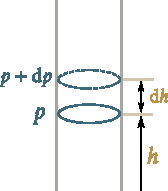
\includegraphics[scale=1.0]{figures/ch_10/fig_10_7.pdf}
			\caption[]{}
			\label{fig:10_7}
		\end{center}
	\end{minipage}
	\hspace{-0.05cm}
	\begin{minipage}[t]{0.5\linewidth}
		\begin{center}
			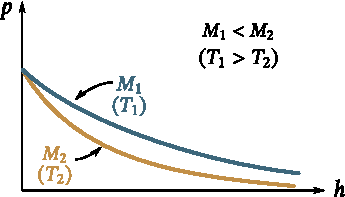
\includegraphics[scale=1.0]{figures/ch_10/fig_10_8.pdf}
			\caption[]{}
			\label{fig:10_8}
		\end{center}
	\end{minipage}
\end{figure}

We indicated in Sec.~\ref{sec:10_8} that air differs only slightly from an ideal gas in its behaviour in conditions close to standard ones. Therefore, the density of air can be calculated by \eqn{10_22}. The introduction of this equation into \eqn{10_68} yields
\begin{equation}\label{eq:10_69}
	\deriv{p} = -\frac{Mpg}{RT}\,\deriv{h}.
\end{equation}

\noindent
The quantity $M$ in this equation numerically equals the average molecular mass of air determined with account taken of the content of nitrogen, oxygen, and other gases in it. It can be seen from \eqn{10_69} that
\begin{equation}\label{eq:10_70}
	\frac{\deriv{p}}{p} = -\frac{Mg}{RT}\,\deriv{h}.
\end{equation}

\noindent
The temperature $T$ is a function of $h$. If we know the form of this function, we can integrate \eqn{10_70} and find how $p$ depends on $h$. For a constant temperature, \ie, for an isothermal atmosphere, integration of \eqn{10_70} leads to the expression
\begin{equation*}
	\ln({p}) = -\frac{Mgh}{RT} + \ln{C}
\end{equation*}

\noindent
where $C$ is a constant (it is convenient here to denote the integration constant by $\ln{C}$). Raising this expression to a power yields
\begin{equation*}
	p = C\,\exp\left(- \frac{Mgh}{RT} \right).
\end{equation*}

\noindent
Introducing $h=0$ into this expression, we find that $C=p_0$, where $p_0$ is the pressure at the altitude $h=0$.

Thus, for our assumption on constancy of the temperature, the dependence of the pressure on the altitude is given by the formula
\begin{equation}\label{eq:10_71}
	p = p_0\,\exp\left(- \frac{Mgh}{RT} \right).
\end{equation}

\noindent
This is the \textbf{barometric formula}. A glance at it shows that the pressure diminishes with the altitude the more rapidly, the heavier is the gas (the greater is $M$) and the lower is the temperature. Figure~\ref{fig:10_8} shows two curves corresponding to \eqn{10_71}. They can be interpreted either as corresponding to different $M$'s (at the same temperature), or to different $T$'s (at the same values of $M$).
